\chapter{Experimental Setup}
\label{ch:ExperimentalSetup}
% Do not write long version of imu or lidar acronym again
\glslocalunset{imu}
\glslocalunset{lidar}

To evaluate the performance of the proposed methods, different test drives must be conducted using a car with the appropriate sensor setup.
In this chapter the properties of the sensors used during the recordings and their placement on the car are described.
Information about the car and its limitations are described in \cref{sec:car}.
Finally, in \cref{sec:garage}, the different type of ramps and their properties are presented.


\section{Sensors}
\subsection{\glsentryshort{imu}}
\begin{figure}[htb]
    \centering
    \begin{subfigure}[b]{0.4\textwidth}
        \centering
        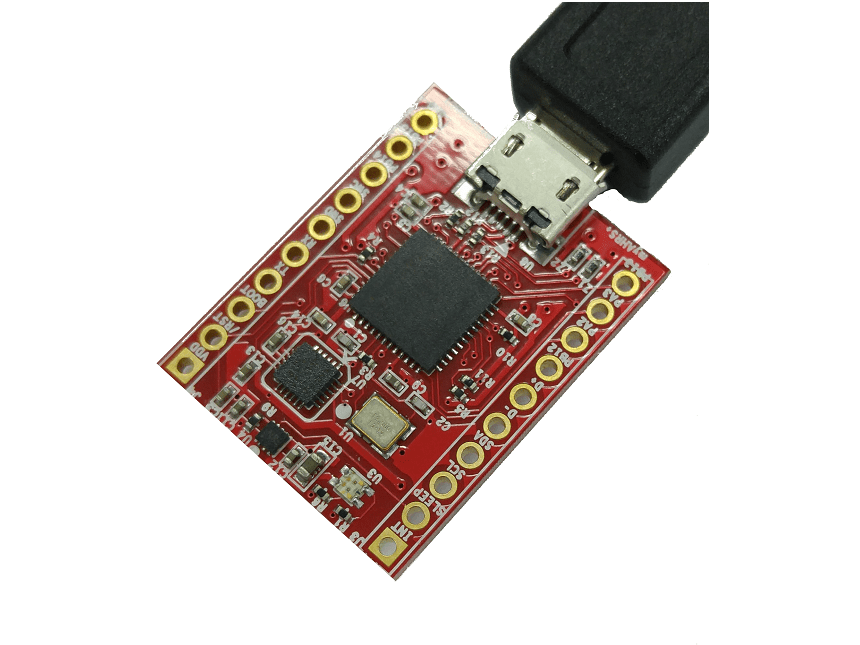
\includegraphics[width=\textwidth]{myAHRS}
        \caption{Withrobot myAHRS+~\cite{Withrobot2017}}
        \label{fig:imu_myahrs}
    \end{subfigure}
    % \hfill
    \begin{subfigure}[b]{0.4\textwidth}
        \centering
        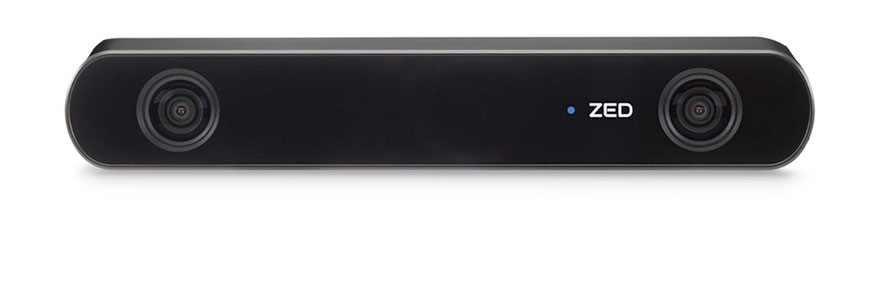
\includegraphics[width=\textwidth]{zed2i}
        \caption{Stereolabs ZED 2i camera~\cite{Stereolabs2019}}
        \label{fig:imu_zed}
    \end{subfigure}
    \caption[\glsentryshortpl{imu} used in the experiment]{The two \acrshortpl{imu} which will be used for the recordings. The Stereolabs ZED 2i camera has an integrated \acrshort{imu}.}
    \label{fig:imus_used}
\end{figure}
Two different \glspl{imu} will be used for the experiment.

The first one being the Withrobot myAHRS+ (see \cref{fig:imu_myahrs}), a low-cost high performance \gls{ahrs}.
An \gls{ahrs} contains an \gls{imu} and outputs the raw measurements of the sensors, but also has an on-board processing system which estimates attitude and heading.
The myAHRS+ uses an extended Kalman filter for the estimation and outputs the estimation in quaternion form and also in Euler angles.

The second \gls{imu} used during the experiment is integrated in the Stereolabs ZED 2i stereo camera and is also an \gls{ahrs}.
A picture of the camera can be seen in \cref{fig:imu_zed}.
More information about the ZED 2i camera and their other integrated sensors and functionalities will be described in \cref{ssec:camera}.

Both sensors are connected to a computer via USB.
The specifications of each \gls{imu} is provided in \cref{tab:imu_datasheets}.
Because no information about the noise density or random walk of the myAHRS+ \gls{imu} could be found, a manual estimation of the error was done using the package \texttt{allan\_variance\_ros}~\footnote{\url{https://github.com/gaowenliang/imu_utils}}.
It analyzes the Allan variance from \gls{imu} measurement data recorded over a two-hour period, during which the \gls{imu} has not been moved.
The smaller values of the ZED 2i \gls{imu} indicate, that it is the better sensor.
\begin{table}[ht]
    \centering
    \caption[Comparison of the two used \glsentryshortpl{imu}]{Comparison of the two used \acrshortpl{imu}~\cite{Withrobot2017, Stereolabs2019}.}
    \label{tab:imu_datasheets}
    \begin{tabular}[t]{lrrc}
        \toprule
        \textbf{Property}           & \textbf{myAHRS+} & \textbf{ZED 2i \gls{imu}} & \textbf{Unit}                                               \\
        \midrule
        Accelerometer range         & $\pm16$          & $\pm8$                    & \si{g}                                                      \\
        Gyroscope range             & $\pm2000$        & $\pm1000$                 & \si{\degree\per\second}                                     \\
        Magnetometer range          & $\pm1200$        & $\pm2500$                 & \si{\micro\tesla}                                           \\
        Rate                        & \SI{100}         & \SI{400}                  & \si{\hertz}                                                 \\
        Accelerometer noise density & \SI{4.502e-3}{}  & \SI{1.148e-3}{}           & \si{\frac{\metre}{\second\squared}\frac{1}{\sqrt{\hertz}}}  \\
        Accelerometer random walk   & \SI{7.337e-5}{}  & \SI{6.458e-5}{}           & \si{\frac{\metre}{\second\cubed}\frac{1}{\sqrt{\hertz}}}    \\
        Gyroscope noise density     & \SI{1.674e-4}{}  & \SI{8.254e-5}{}           & \si{\frac{\radian}{\second}\frac{1}{\sqrt{\hertz}}}         \\
        Gyroscope random walk       & \SI{5.042e-6}{}  & \SI{1.632e-7}{}           & \si{\frac{\radian}{\second\squared}\frac{1}{\sqrt{\hertz}}} \\
        \bottomrule
    \end{tabular}
\end{table}


\subsection{\glsentryshort{lidar}}
\begin{figure}[htbp]
    \centering
    \begin{subfigure}{0.4\textwidth}
        \centering
        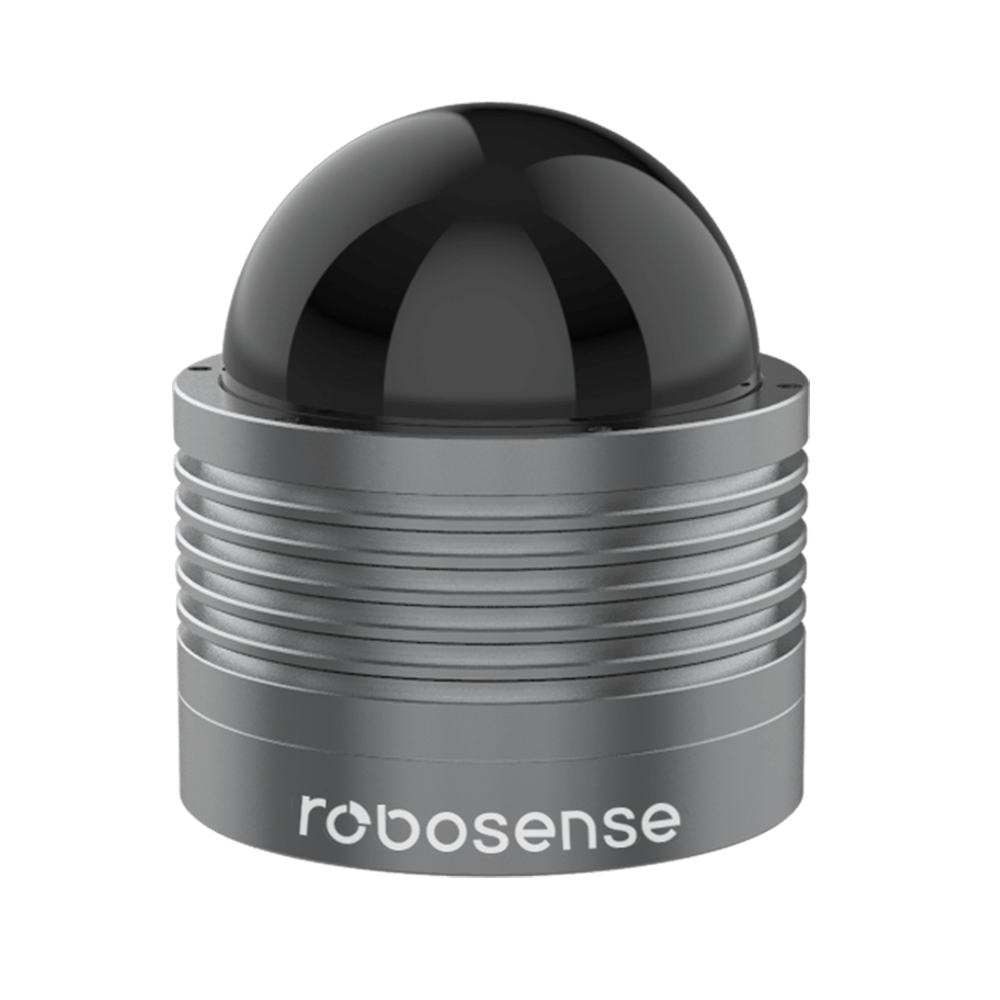
\includegraphics[width=\textwidth]{Robosense}
        \caption{Robosense RS-Bpearl~\cite{RoboSense2020}}
        \label{fig:lidar_robosense}
    \end{subfigure}
    % \hfill
    \begin{subfigure}{0.4\textwidth}
        \centering
        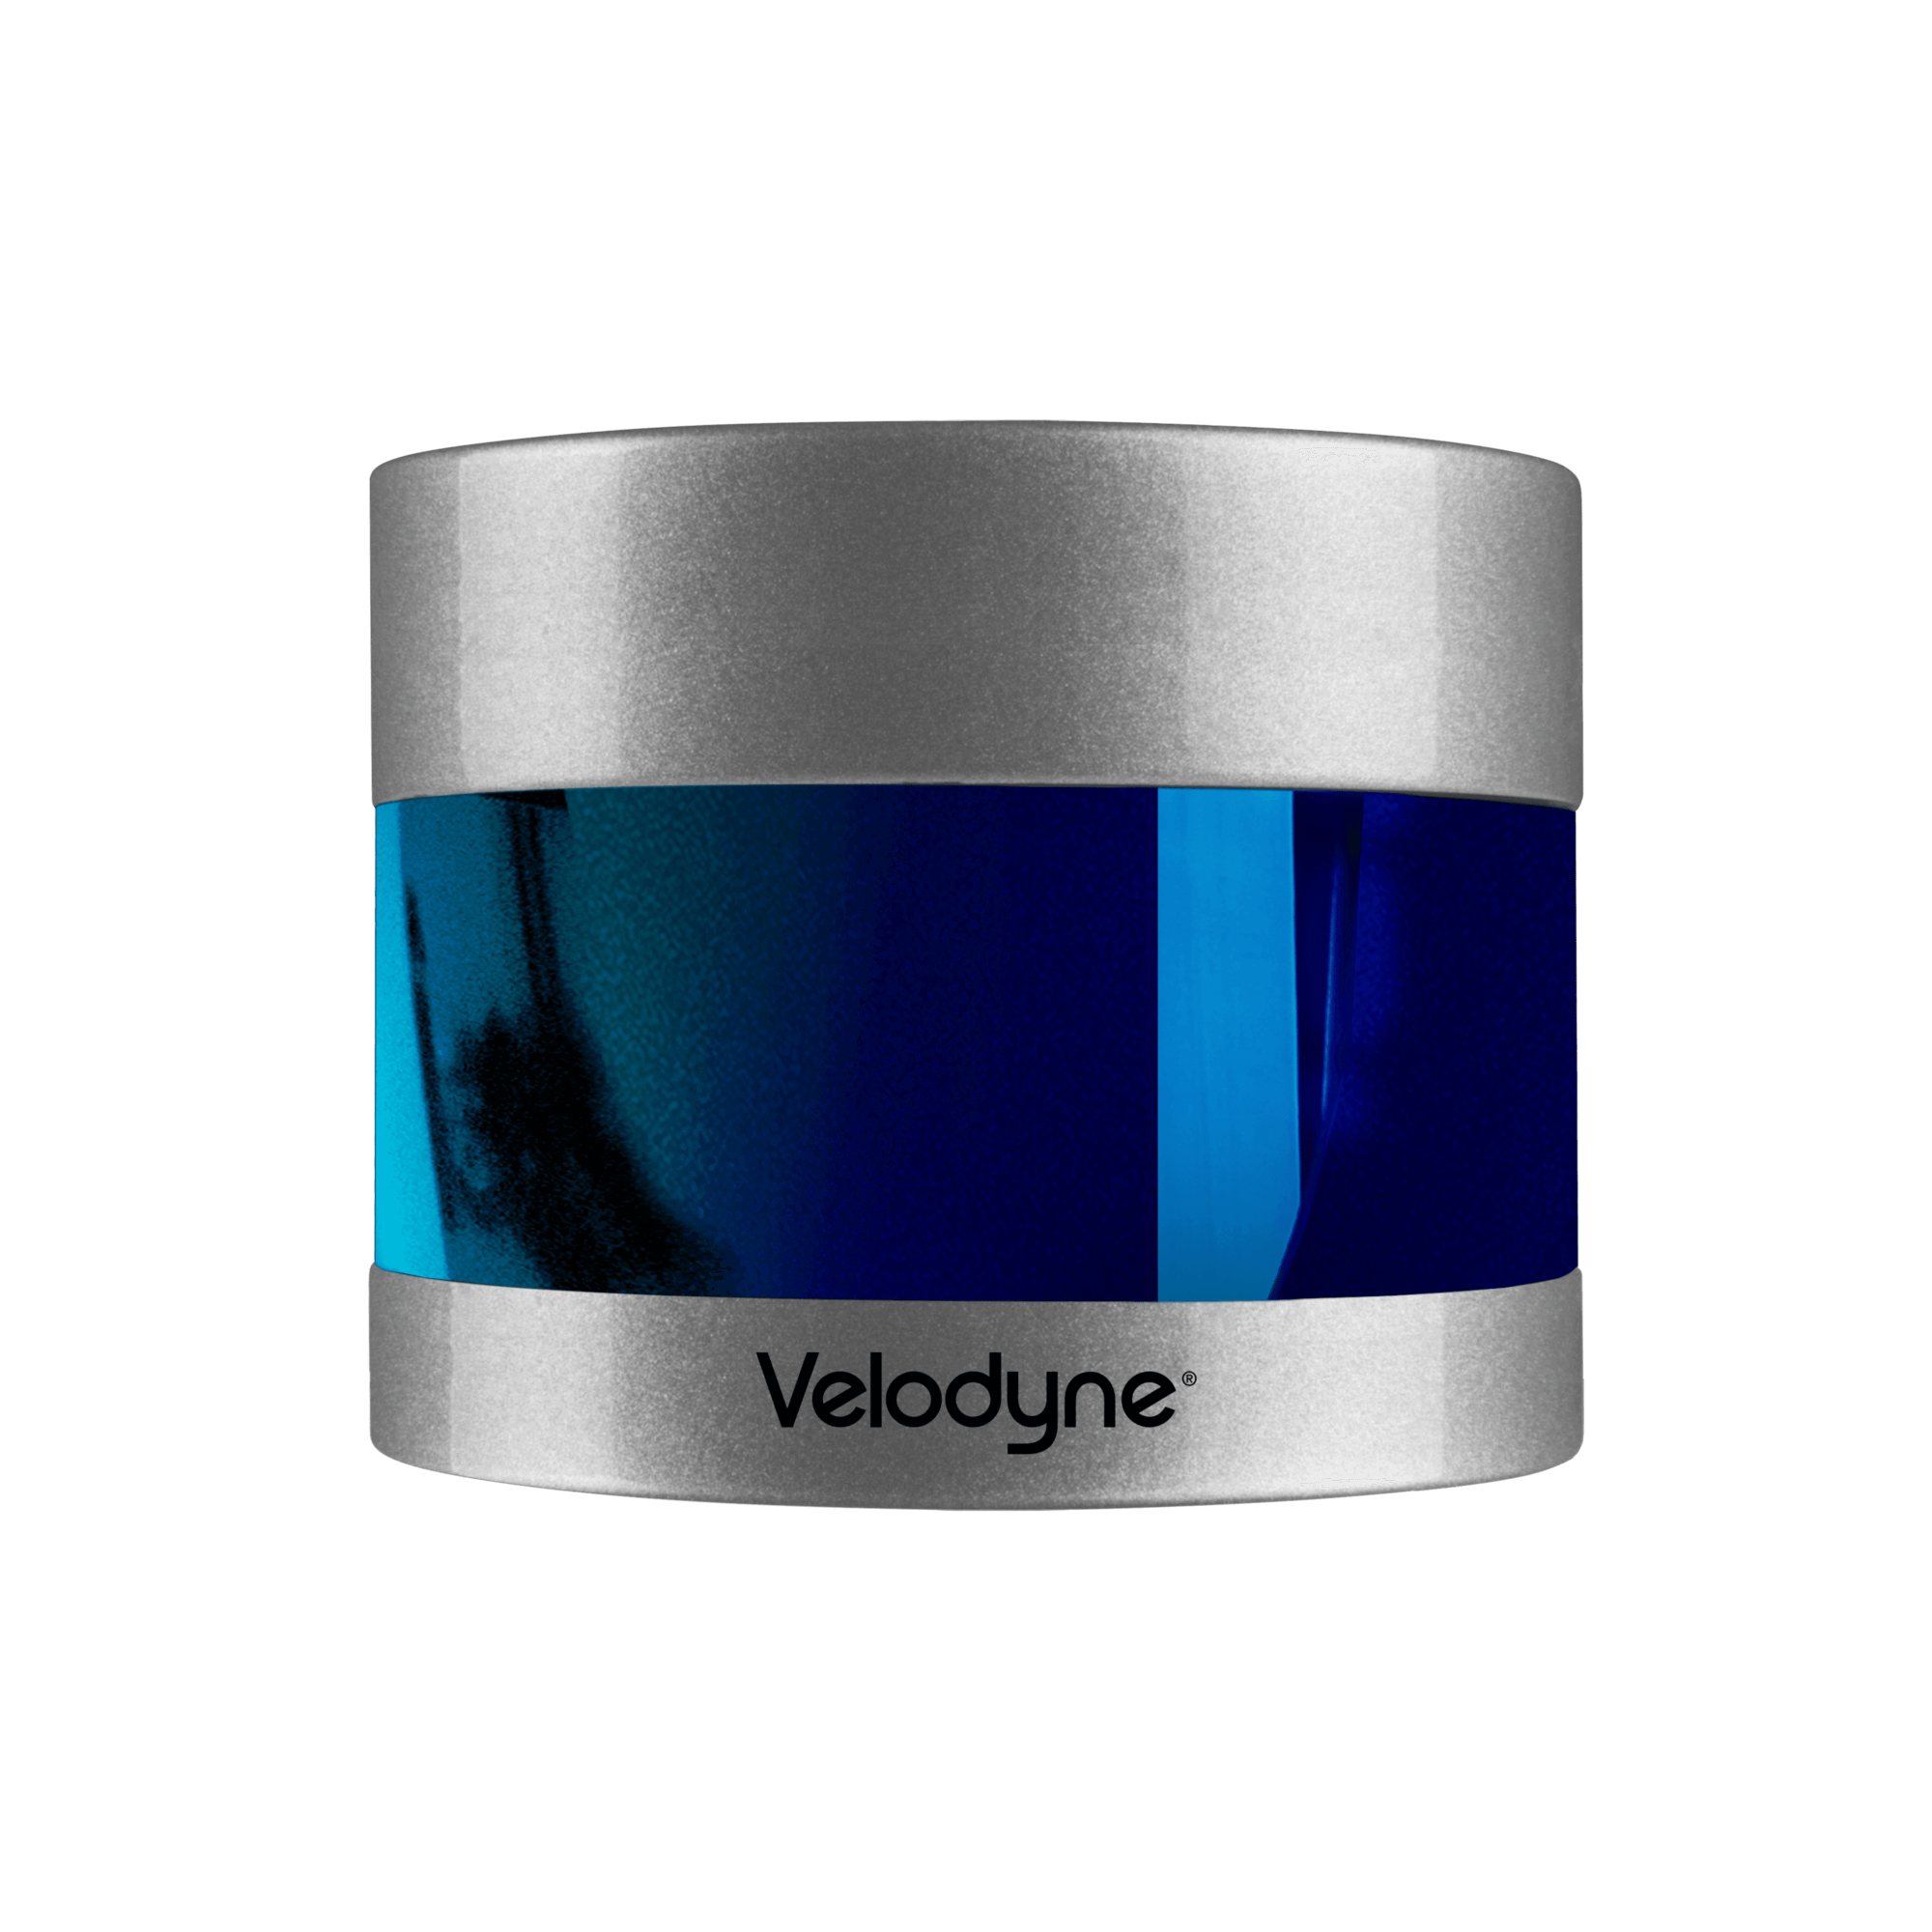
\includegraphics[width=\textwidth]{Velodyne}
        \caption{Velodyne Ultra puck~\cite{Velodyne2018}}
        \label{fig:lidar_velodyne}
    \end{subfigure}
    \caption[\glsentryshortpl{lidar} used in the experiment]{The two \acrshortpl{lidar} which will be used for the recordings.}
    \label{fig:lidars_used}
\end{figure}
Two different \glspl{lidar} will be used during the experiment.
The RS-Bpearl and the Velodyne UltraPuck, see \cref{fig:lidars_used}.
The most relevant specifications of the two \glspl{lidar} are listed in \cref{tab:lidar_datasheets}.
Both are mechanical \glspl{lidar} and have the same number of laser channels, but the Velodyne has a significantly better vertical resolution, due to the smaller vertical \gls{fov}.
This is because the RS-Bpearl is intended to be used as near-field blind-spots detection \gls{lidar} mounted on the side where coverage is more important than resolution.
The Velodyne UltraPuck on the other hand has been specifically designed for being mounted on the roof and hence also has a greater range.

Both \glspl{lidar} need an external power supply and the data transfer to the PC is done via Ethernet connection.
Due to the setup of the test car it is only possible to mount one \gls{lidar} at a time.
\begin{table}[ht]
    \centering
    \caption[Comparison of the two used \glsentryshortpl{lidar}]{Comparison of the two used \acrshortpl{lidar}s~\cite{RoboSense2020, Velodyne2018}.}
    \label{tab:lidar_datasheets}
    \begin{tabular}[t]{lrrc}
        \toprule
        \textbf{Property}     & \textbf{RS-Bpearl}   & \textbf{Velodyne Ultra Puck}    & \textbf{Unit}     \\
        \midrule
        Channels              & 32                   & 32                              &                   \\
        Points per second     & \num{576000}         & \num{600000   }                 &                   \\
        Laser wavelength      & \SI{905}{}           & \SI{903}{}                      & \si{\nano\metre}  \\
        Frame rate            & \SIrange{10}{20}{}   & \SIrange{5}{20}{}               & \si{\hertz}       \\
        Range                 & \SI{100}{}           & \SI{200}{}                      & \si{\metre}       \\
        Range accuracy        & $\pm\SI{3}{}$        & $\pm\SI{3}{}$                   & \si{\centi\metre} \\
        Horizontal \gls{fov}  & \SI{360}{}           & \SI{360}{}                      & \si{\deg}         \\
        Vertical \gls{fov}    & \SI{90}{}            & \SI{40}{} (\SIrange{-25}{15}{}) & \si{\deg}         \\
        Horizontal resolution & \SIrange{0.2}{0.4}{} & \SIrange{0.1}{0.4}{}            & \si{\deg}         \\
        Vertical resolution   & \SI{2.81}{}          & \SI{0.33}{}                     & \si{\deg}         \\
        \bottomrule
    \end{tabular}
\end{table}


\subsection{Camera}
\label{ssec:camera}
The ZED 2i camera from Stereolabs as seen in \cref{fig:imu_zed} will be used during the experiment to record the camera image.
The camera has two horizontally displaced lenses, allowing for stereo vision and thus also depth estimation.
A barometer, temperature sensor and an \gls{imu} are integrated as well.
It also provides many more features such as 3D positional tracking, mapping, object detection and point cloud generation.

Because only one image is needed, only the image of the left camera is used.
The resolution is set to 1280x720 and a frame rate per second of 30 is used.
The camera is connected to the PC through USB.



\section{Sensor Placement}
To ensure the best possible performance of the system, the sensors must be placed in a specific way.
The \gls{imu} must be placed on a rigid point of the car, such that the \gls{imu}'s position always stays the same relative to the car.
Other than that it should also be placed in the transversal center of the car to guarantee that the centripetal acceleration is not skewed towards one side when driving around a corner.
The placement of the \gls{imu} integrated in the ZED 2i camera is limited, because the camera images are needed as well.
It was placed on the roof of the car, which is sturdy enough to not be suspect to flexion, while also allowing for a good \gls{fov} for the camera.
The myAHRS+ \gls{imu} was mounted on the floor of the car trunk.

The \gls{lidar} is placed on top of the car, to get a greater \gls{fov}.
The pitch angle $\beta$ at which the \gls{lidar} will be mounted should be chosen such that the number of points in the area at the beginning of the ramp are maximized.
This allows for the most accurate distinction between planes of different inclination angles.
Because the distance to the ramp is not constant due to the movement of the car, the optimization can only be done for a specific distance.
The coordinates at which the lasers hit the ground and ramp depend on the height of the \gls{lidar} $h_\mathrm{l}$, the distance to the ramp $d$, the angle of the ramp \gls{ramp_ang}, the angle $\beta$ at which the \gls{lidar} has been mounted on the car and finally on the vertical resolution $\epsilon$ and \gls{fov} of the \gls{lidar}.
A visualization of the different variables can be seen in \cref{fig:tikz_lidar_mount}.
\begin{figure}[htb]
    \centering
    \documentclass[12pt]{standalone}
\usepackage{tikz}
\usepackage{tikz-dimline}		% Dimension (measure) lines for TikZ
\usetikzlibrary{angles, calc, decorations.pathmorphing, quotes, spy}

\begin{document}
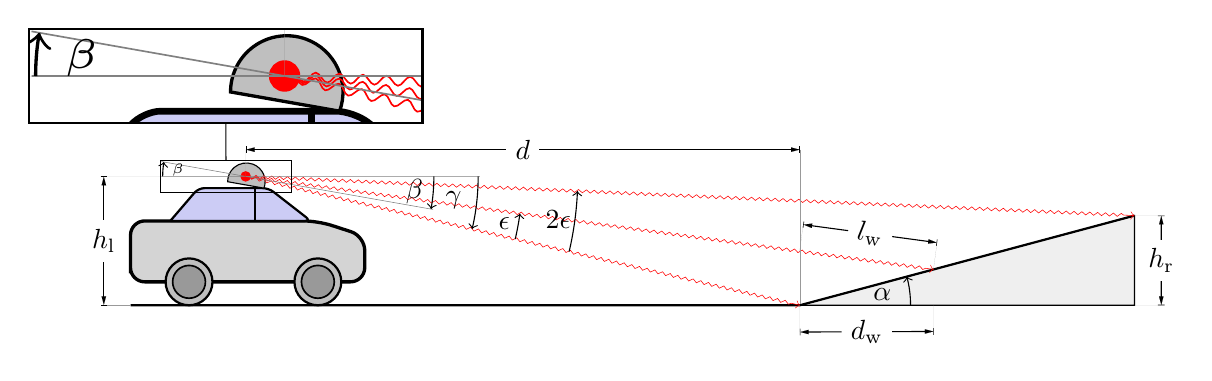
\begin{tikzpicture}[scale=0.85, spy using outlines={black, rectangle, magnification=3, width=5cm, height=1.2cm, connect spies}]
        % Define/Calc ramp parameters
        % Ramp length
        \def\rl{5};
        % Ramp angle [deg]
        \def\ra{15};
        % Ramp height
        \def\rh{{tan(\ra)*\rl}};
        % Distance of measurement line
        \def\dd{.4cm}

        % RAMP
        % Define the points
        % Left point
        \coordinate (A) at (0,0);
        % Lower right point
        \coordinate (B) at ($(A) + (\rl,0)$);
        % Upper right point
        \coordinate (C) at ($(B) + (0,\rh)$);

        % Draw and fill ramp
        \filldraw[draw=black, fill=lightgray!25] (A) -- (B) -- (C) -- cycle;
        % Draw ramp angle
        \path (A) -- (B)
        pic[draw, ->, angle radius=40pt,
                        angle eccentricity=0.75, "$\alpha$"]{angle=B--A--C};

        % Most left point at ground level
        \coordinate (D) at ($(A) + (-10,0)$);
        % Ground line
        \draw [thick] (D) -- (A) -- (C);


        % CAR
        \begin{scope}[scale=0.7]
                % Car height
                \def\ch{2}
                % Car length
                \def\cl{5}
                % Car body height
                \def\bh{\ch*0.65}
                % Roof length
                \def\rl{\cl*0.6}
                % Roof height
                \def\rh{\ch*0.35}
                % Anchor point of car body (lower left)
                \coordinate (b) at ($(D) + (0,0.5)$);
                % Offset to roof and wheels
                \coordinate (r) at ($(b) +(\cl*0.17,\ch*0.65)$);
                \coordinate (w) at ($(b) + (\cl*0.25,0)$);

                % Body
                \draw[black, fill=black!17, rounded corners=1.2ex, very thick]
                (b) -- ++(0,\bh) -- ++(\cl*1/5,0) --  ++(\cl*3/5,0) -- ++(\cl*1/5,-\bh*0.25)
                -- ++(0, -\bh*0.75) -- (b) -- cycle;
                % Roof
                \draw[very thick, rounded corners=0.5ex, fill=black!20!blue!20!white,thick]
                (r) -- ++(0.2*\rl,\rh) -- ++(0.5*\rl,0) -- ++(0.3*\rl,-\rh) -- (r);
                \draw[thick] (r)++(\rl*0.6,0) -- ++(0,\rh);

                % Wheels
                \draw[draw=black,fill=gray!50,thick] (w) circle (.5);
                \draw[draw=black,fill=gray!50,thick] (w) ++(\cl*0.55,0) circle (.5);
                % Inner wheels
                \draw[draw=black,fill=gray!80,semithick] (w) circle (.35);
                \draw[draw=black,fill=gray!80,semithick] (w) ++(\cl*0.55,0) circle (.35);

                % Lidar
                % Lidar pitch angle
                \def\lpa{10};
                \draw[black, fill=gray!50] ($(r) + (\cl*0.40,\rh)$) coordinate (le) arc(-\lpa*2:180:0.4) --cycle;

                % Car middle point
                \coordinate (m) at (\cl*0.5, \bh*0.5);
                % Lidar middle point
                \coordinate (lm) at ($(le) + (-0.39,0.25)$);
                \filldraw[red] (lm) circle(.1);
                \coordinate (idk) at ($(A)!0.4!(C)$);

                % Laser lines
                \draw[->,color=red,very thin,decorate,decoration={snake,amplitude=.2mm,segment length=1mm,post length=1mm}] (lm) -- (A)
                pic[draw, black, ->, thin, angle radius=100pt, angle eccentricity=0.95,
                                "$\epsilon$"]{angle=A--lm--idk};
                \draw[->,color=red,very thin,decorate,decoration={snake,amplitude=.2mm,segment length=1mm,post length=1mm}] (lm) -- ($(A)!0.4!(C)$);
                \draw[->,color=red,very thin,decorate,decoration={snake,amplitude=.2mm,segment length=1mm,post length=1mm}] (lm) -- ($(A)!1!(C)$)
                pic[draw, black, ->, thin, angle radius=120pt, angle eccentricity=0.95,
                                "$2\epsilon$"]{angle=A--lm--C};


                % lidar mount angle
                % Length of angle helper line
                \def\hl{4};
                \def\hll{1.8};
                \coordinate (bleb) at ($(lm) + (\hl+1, 0)$);
                \coordinate (blab) at ($(lm) + (\hl, -{tan{\lpa}*\hl})$);
                \coordinate (blub) at ($(lm) + (-\hll, 0)$);
                \coordinate (blob) at ($(lm) + (-\hll, +{tan{\lpa}*\hll})$);
                \draw[draw=gray, very thin] (blub) -- (lm) -- (blob)
                pic[draw, black, thin, <-, angle radius=30pt,
                                angle eccentricity=0.82, "\tiny $\beta$"]{angle=blob--lm--blub};
                \draw[draw=gray, very thin] (bleb) -- (lm) -- (blab)
                pic[draw, black, thin, <-, angle radius=68pt,
                                angle eccentricity=0.9, "$\beta$"]{angle=blab--lm--bleb};
                \path (bleb) -- (lm) -- (A)
                pic[draw, <-, thin, angle radius=84pt,
                                angle eccentricity=0.9, "$\gamma$"]{angle=A--lm--bleb};

        \end{scope}

        % \filldraw[green] (idk) circle(.2);
        \dimline[extension start length=\dd, extension end length=\dd+1.9cm] {($(lm)+(0,\dd)$)}{($(lm -| A)+(0,\dd)$)}{$d$};
        % \dimline[extension start length=-\dd, extension end length=-\dd] {($(A)+(0,-\dd)$)}{($(B)+(0,-\dd)$)}{$l_\mathrm{r} $};
        \dimline[extension start length=-\dd, extension end length=-\dd, label style={sloped=false}] {($(B)+(\dd,0)$)}{($(C)+(\dd,0)$)}{$h_\mathrm{r}$};
        \dimline[extension start length=\dd, extension end length=\dd+1.7cm, label style={sloped=false}] {($(D)+(-\dd,0)$)}{($(lm -| D)+(-\dd,0)$)}{$h_\mathrm{l} $};

        % \dimline[extension start length=\dd, extension end length=-\dd] {($(idk)+(\dd,0)$)}{($(idk)+(\dd,-0.53)$)}{};
        % \dimline[extension start length=0, extension end length=0, label style={right, fill=none, sloped=false}] {(idk)}{($(idk)+(0,-0.53)$)}{$h_\mathrm{w}$};
        \dimline[extension start length=-\dd, extension end length=-\dd] {($(A)+(0,-\dd)$)}{($(idk)+(0,-\dd-15)$)}{$d_\mathrm{w} $};
        \dimline[extension start length=\dd, extension end length=\dd] {($(A)+(0.05,-\dd+\dd+34.3)$)}{($(idk)+(0.05,\dd)$)}{$l_\mathrm{w} $};

        % \spy[black] on ($(lm) + (-0.42, 0)$) in node at (3,4);
        \spy on ($(lm) + (-0.25, 0)$) in node at ($(lm) + (-0.3, 1.5)$);

\end{tikzpicture}
\end{document}
    \caption[\glsentryshort{lidar} placement on the car]{Calculation of the best mounting angle of the \acrshort{lidar} on the car. The used variables are described in \cref{tab:lidar_mount}.}
    \label{fig:tikz_lidar_mount}
\end{figure}
The coordinates at which the laser lines of the \gls{lidar} hit the ground can be calculated in the following way.

The angle $\kappa$ between the plane parallel to the ground at \gls{lidar} height and each laser wave is defined as
\begin{equation}
    \kappa = \beta - i\epsilon
\end{equation}
with $i \in [0,1,2,\dots,n]$ being the laser channel ID starting from the lowest opening angle and going to the highest and $n$ being the number of laser channels.
On flat ground the distance at which the laser waves hit the ground can be calculated by
\begin{equation}
    d_\mathrm{hit,ground}  = \tan(\ang{90} - \kappa) h_\mathrm{l}.
    \label{eq:ground_points}
\end{equation}
With a ramp, the assumption from \cref{eq:ground_points} does not hold anymore.
The light does not travel as far.
The height above ground, when the light is at the beginning of the ramp can be calculated by
\begin{equation}
    h_\mathrm{w,start} = h_\mathrm{l} - d\tan(\kappa).
\end{equation}
The distance $l_\mathrm{w}$ which the light travels from the beginning of the ramp to the contact point with the ramp can be calculated using the law of sines
\begin{align}
    l_\mathrm{w} & = \frac{h_\mathrm{w,start} }{\sin(\gls{ramp_ang} + \kappa)} \sin(\ang{90} - \gls{ramp_ang}) \nonumber \\
                 & = -\frac{h_\mathrm{w,start} }{\sin(\gls{ramp_ang} + \kappa)} \cos(\gls{ramp_ang}).
\end{align}
The traveled distance along the x-axis from the start of the ramp to the contact point is then
\begin{align}
    d_\mathrm{w} & = l_\mathrm{w} \sin(\ang{90} - 2\gls{ramp_ang} - \kappa) \nonumber \\
                 & = -l_\mathrm{w} \cos(2\gls{ramp_ang} + \kappa).
\end{align}
Putting everything together, the total x distance from the \gls{lidar} to the contact point on the ramp can be calculated by
\begin{align}
    d_\mathrm{hit,ramp} & = d + d_\mathrm{w}                                                                                    \nonumber               \\
    d_\mathrm{hit,ramp} & = d + \frac{h_\mathrm{l} - d\tan(\kappa)}{\sin(\gls{ramp_ang} + \kappa)} \cos(\gls{ramp_ang}) \cos(2\gls{ramp_ang} + \kappa).
    \label{eq:final_equation}
\end{align}
Using \cref{eq:ground_points} and \cref{eq:final_equation} and optimizing $\beta$ such that the number of points in the area at the start of the ramp are maximized, the optimal mounting pitch angle $\beta$ for the two \glspl{lidar} has been found with $\beta_\mathrm{velodyne} = \ang{0}$ and $\beta_\mathrm{robos} = \ang{20}$.
The optimization was done for a distance of \SI{10}{\metre} to the ramp.
The angle between the two \glspl{lidar} differs due to the different starting opening angle of \SI{-25}{\degree} and \SI{0}{\degree} for the Velodyne and Robosense respectively, as well as due to the different vertical resolution.
A detailed description of all the variables used for the calculation can be found in \cref{tab:lidar_mount}.
\begin{table}[htb]
    \centering
    \caption[Variables for the calculation of the \glsentryshort{lidar} mounting angle]{Variables used to calculate the optimal mounting angle of the \acrshort{lidar}.}
    \label{tab:lidar_mount}
    \begin{tabular}[t]{clc}
        \toprule
        \textbf{Variable} & \textbf{Description}                                   & \textbf{Unit} \\
        \midrule
        $h_\mathrm{l} $   & \gls{lidar} height above ground                        & \si{\metre}   \\
        $d$               & Distance to ramp                                       & \si{\metre}   \\
        $h_\mathrm{r}$    & Height of ramp                                         & \si{\metre}   \\
        $l_\mathrm{w}$    & Light travel distance from ramp start to contact point & \si{\metre}   \\
        $d_\mathrm{w}$    & Distance from ramp start to contact point              & \si{\metre}   \\
        $\gls{ramp_ang}$  & Ramp angle                                             & \si{\deg}     \\
        $\beta$           & \gls{lidar} mount angle                                & \si{\deg}     \\
        $\kappa$          & Laser line angle                                       & \si{\deg}     \\
        $\epsilon$        & \gls{lidar} vertical resolution                        & \si{\deg}     \\
        $n$               & Number of laser channels                               &               \\
        \bottomrule
    \end{tabular}
\end{table}



\section{Data Recording}
All the sensors are connected to a PC in the car, located in the booth.
A notebook is connected to the PC using a \gls{ssh} connection and is used to start the different sensor streams.
For the communication between the PC and sensors and the recording of the sensor data the \gls{ros} framework is used.
Each sensor publishes its data to a specific topic, which can be subscribed to.
While \gls{ros} allows for real-time running of nodes it is also possible to record all sensor streams and store them in a rosbag.
A rosbag contains the serialized message data and can later be used as a dataset.
The rosbag can be played back in \gls{ros}, simulating the same conditions as during the recording, by publishing the same topics again which were initially subscribed to during the recording.
The different algorithms can then be tested and perhaps improved, without having to physically do the test drive again.



\section{Car}
\label{sec:car}
The car used for the recordings is an eGolf 2017.
Being an electric car it provides better vibration properties than a car with an internal combustion engine, which means that the \gls{imu} measurements are less influenced by external noise.
The car has built in wheel speed sensors, which only provide a signal if used in a special driving mode, in which the output power of the motor is limited.
In this mode, the maximum speed is capped at \SI{5}{\kilo\metre\per\hour} and the torque is limited, such that is not possible to drive a ramp all the way up.
The car can only make it about halfway up.
Because of that, the normal mode was used to drive between different levels.
Before driving down, the mode was switched again to also provide the wheel speed measurements.
A picture of the car with the mounted Velodyne UltraPuck \gls{lidar} and Stereolabs ZED 2i camera can be found in \cref{fig:eGolf}.
The other \gls{lidar} sensors at the side are not used.
\begin{figure}[htb]
    \centering
    \documentclass[11pt]{standalone}
\usepackage{tikz}

\usetikzlibrary{calc}
\begin{document}
\begin{tikzpicture}
    % Include the image in a node
    \node[anchor=south west, inner sep=0] (image) at (0,0) {
        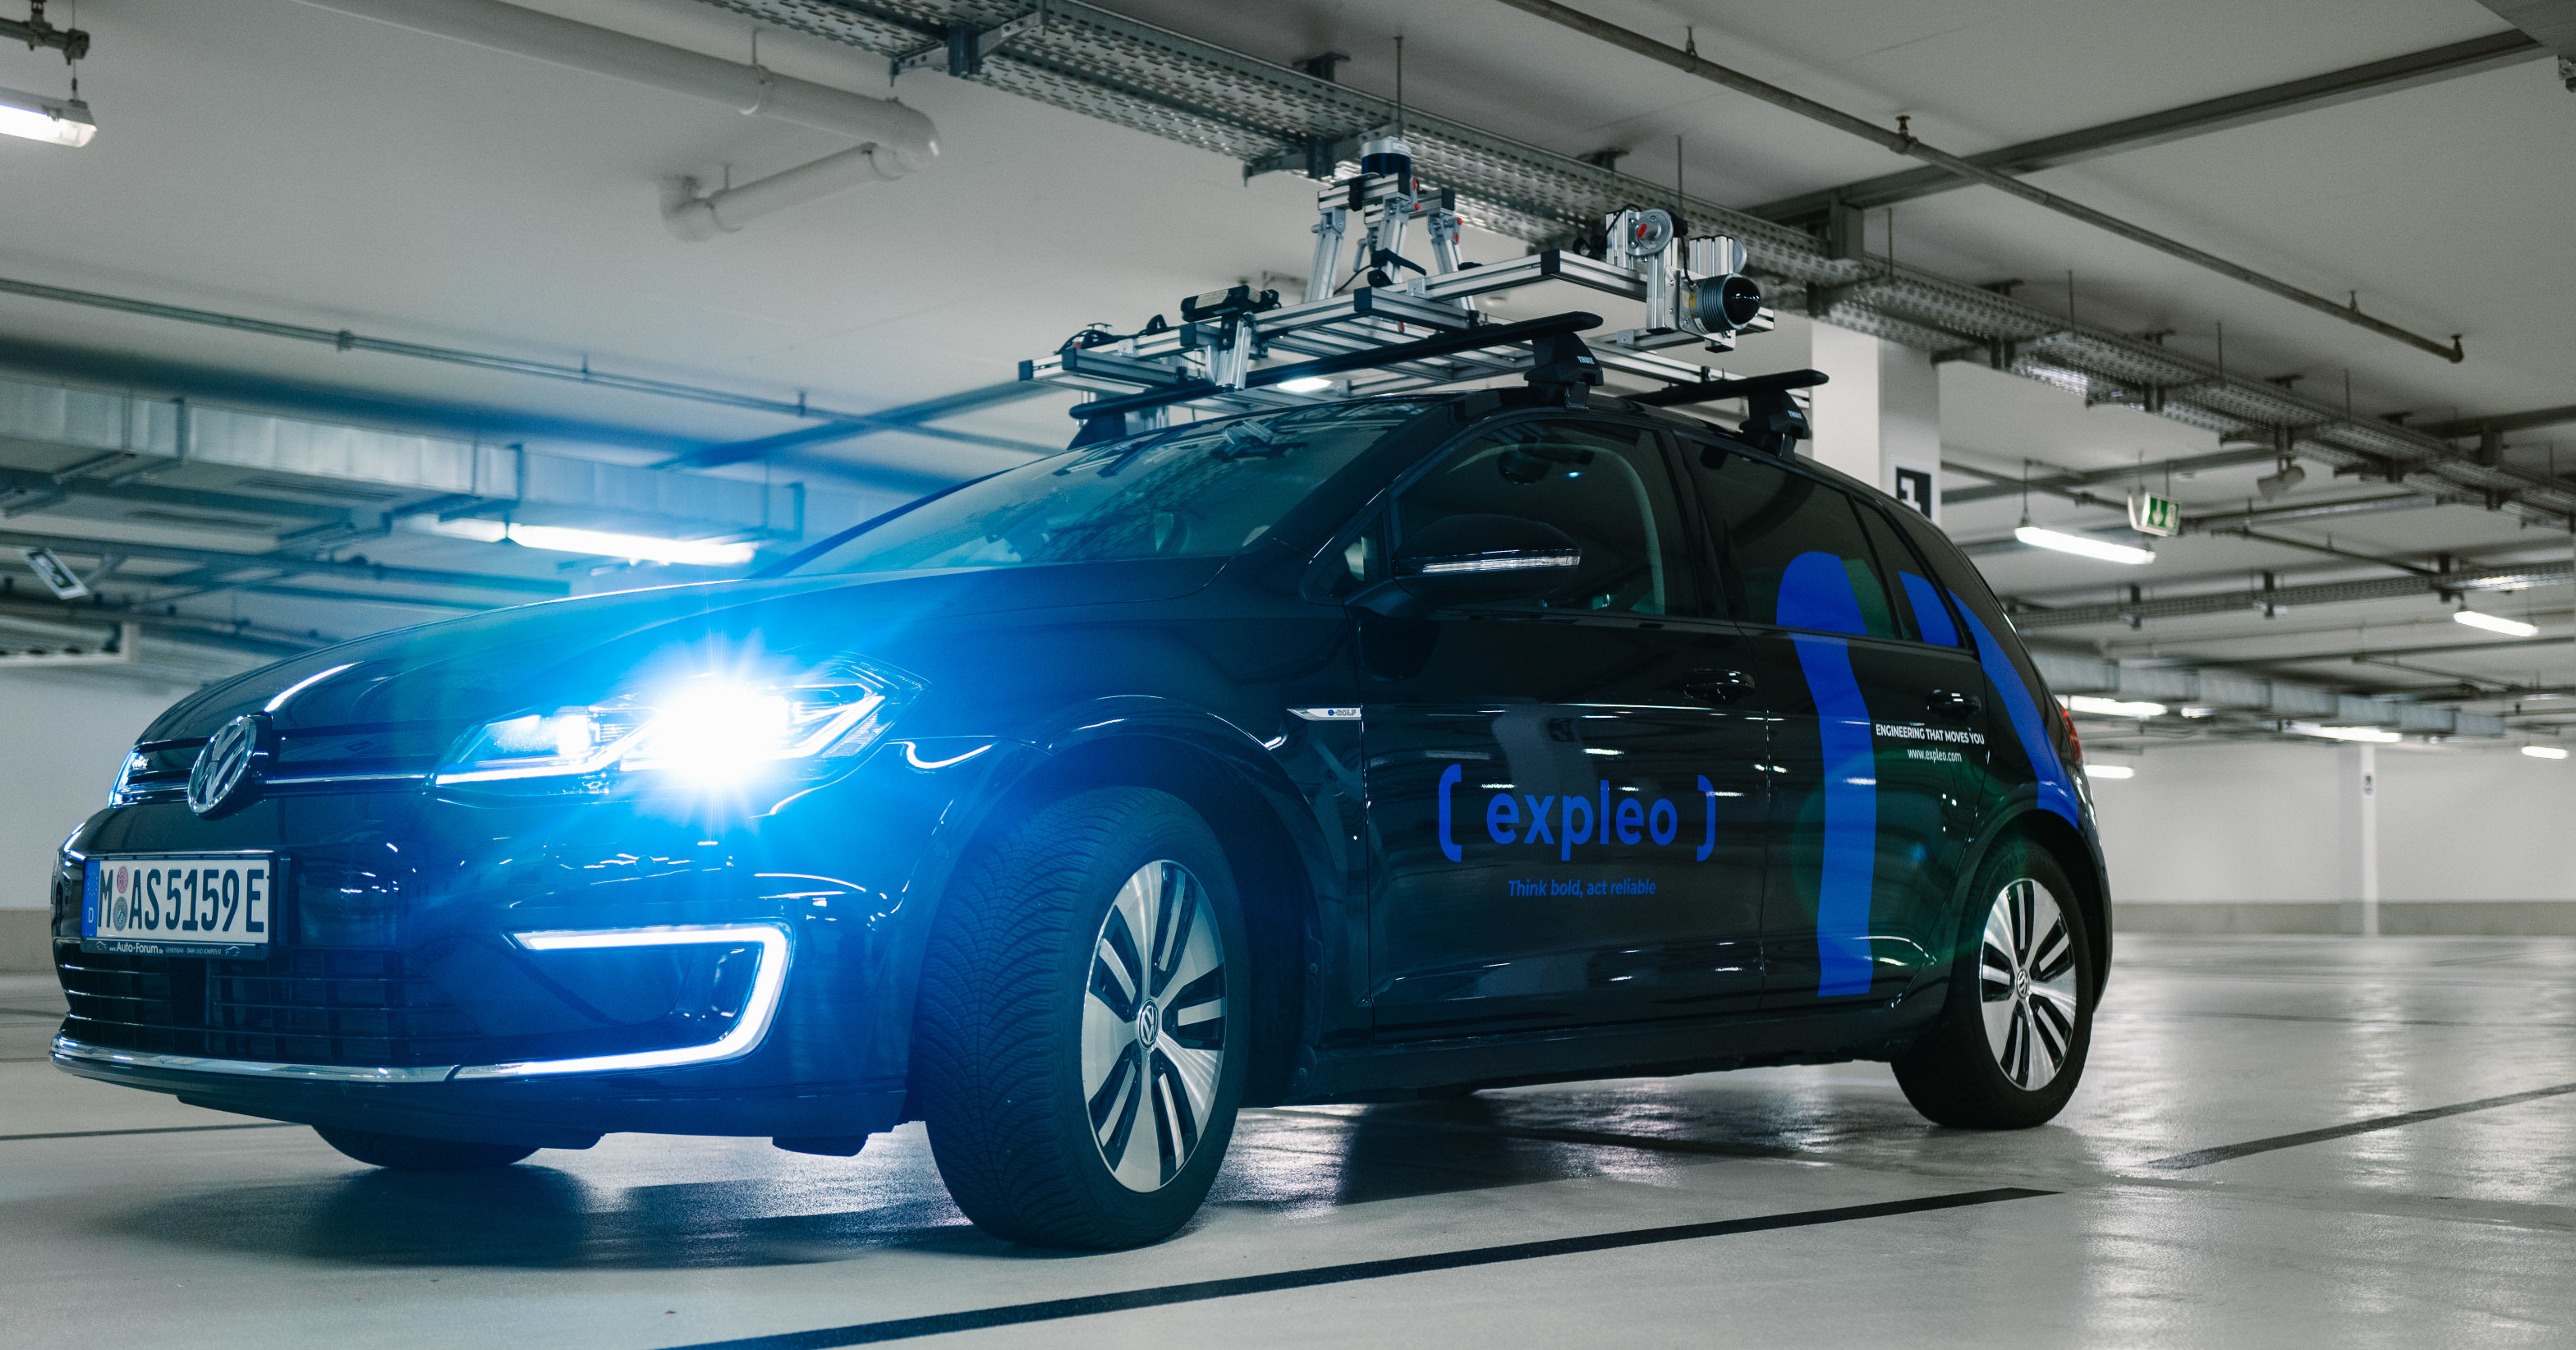
\includegraphics[width=0.77\textwidth]{eGolfPro}
    };

    % Create scope with normalized axes
    \begin{scope}[
            x={($0.1*(image.south east)$)},
            y={($0.1*(image.north west)$)}]

        % Grid (for easier positioning of nodes)
        % \draw[lightgray,step=1] (image.south west) grid (image.north east);
        % % Axes' labels
        % \foreach \x in {0,1,...,10} { \node [below] at (\x,0) {\x}; }
        % \foreach \y in {0,1,...,10} { \node [left] at (0,\y) {\y};}

        % Rectangles to mark sensors
        \draw[green] (5.1,8.2) rectangle (5.7,9.1);
        % node[below left,black,]{1};
        \draw[green] (4.5,7.5) rectangle (5.0,8.0);
        % \draw[very thick,green] (3.3,8.7) rectangle (3.9,9.5);

        % Labels
        \draw[latex-, green] (5.1,8.65) -- ++(-3.4,0)
        node[right,black,fill=white, rounded corners=.07cm]{\footnotesize LiDAR};
        \draw[latex-, green] (4.5,7.7) -- ++(-2.8,0)
        node[right,black,fill=white, rounded corners=.07cm]{\footnotesize Camera \& IMU};


    \end{scope}

\end{tikzpicture}
\end{document}
    \caption[Car with mounted sensors]{The car used for the recordings with the full sensor setup mounted on the roof.}
    \label{fig:eGolf}
\end{figure}



\section{Garage}
\label{sec:garage}
To prevent an overfitting of the model it is important to have different test scenarios.
The garage in which the car is normally parked has different types of ramps, which are shown in \cref{fig:all_ramps}.
The properties of each ramp are described in \cref{tab:ramp_properties}.
The values were measured by inspecting the point cloud generated by the \gls{lidar}.
The width of the ramp is measured between the side wall and the railing, and not between the two curbsides.
Because the ramps do not have a constant angle, because the change of the angle gradually increases, decreases and then increases again, the average angle of the ramps is used.
\begin{figure}[htb]
    \begin{subfigure}{.24\linewidth}
        \centering
        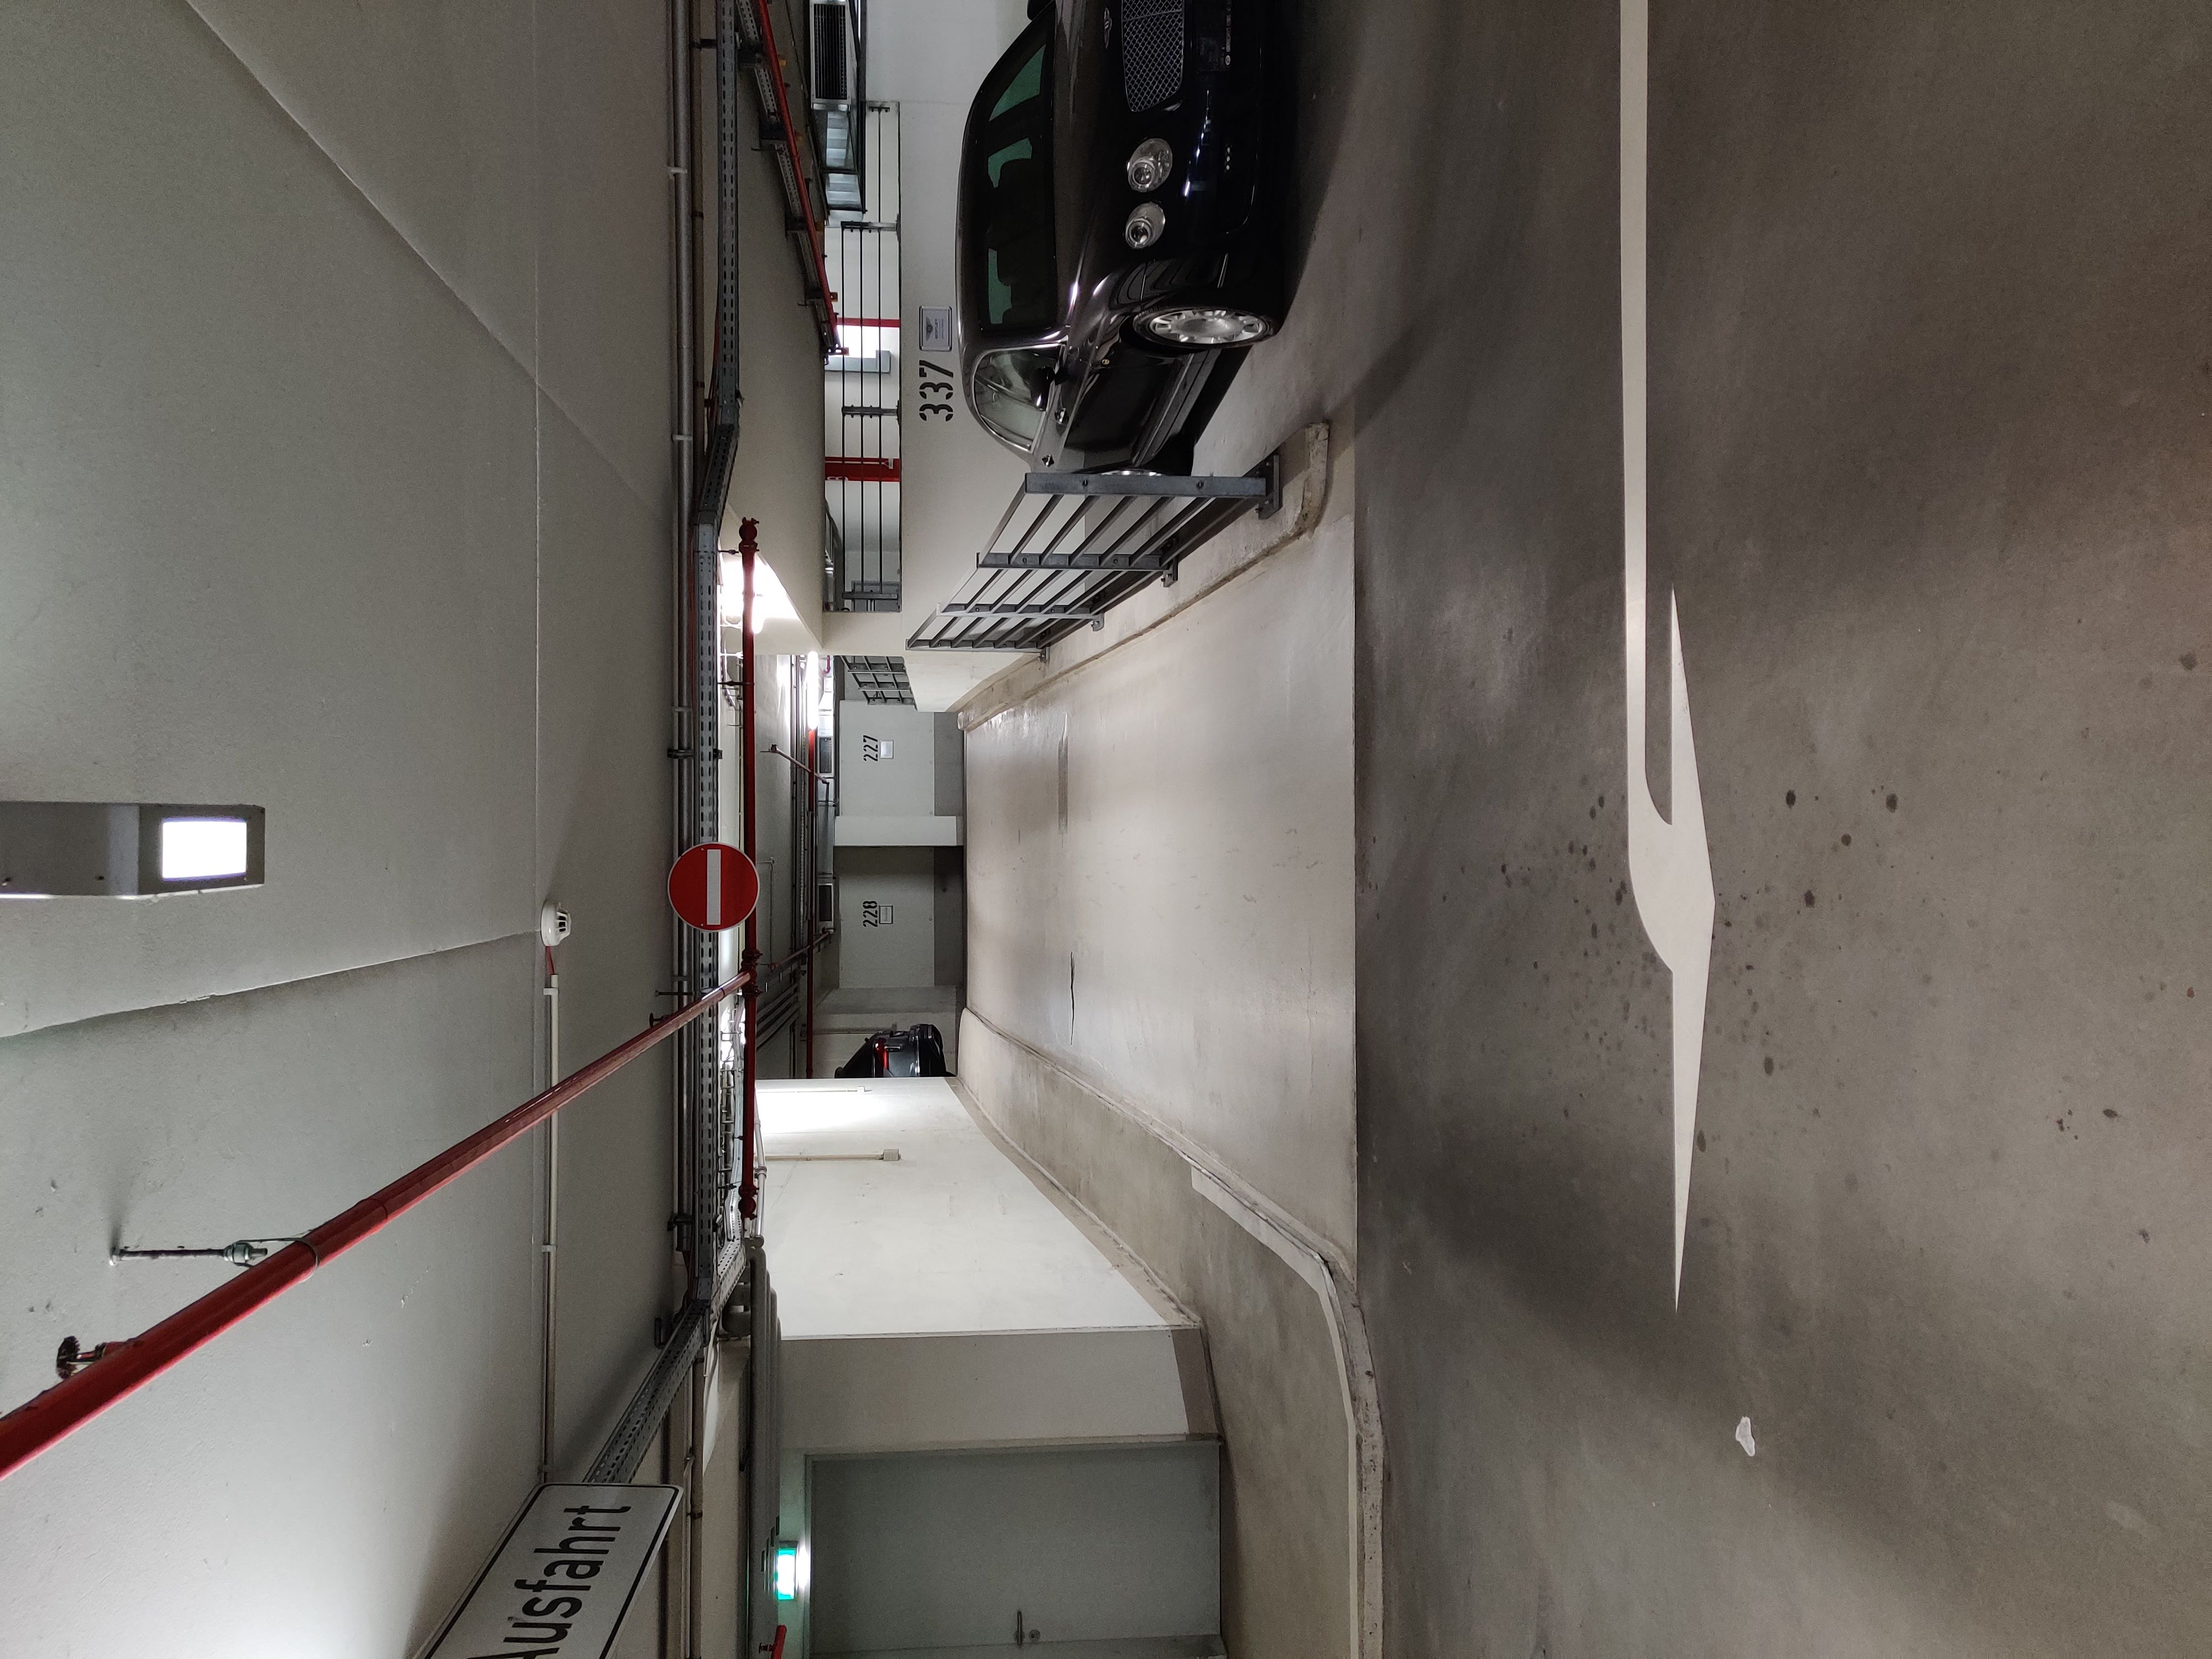
\includegraphics[angle=-90, width=1\linewidth]{RampA.jpg}
        \caption{}
    \end{subfigure}
    \hfill
    \begin{subfigure}{.24\linewidth}
        \centering
        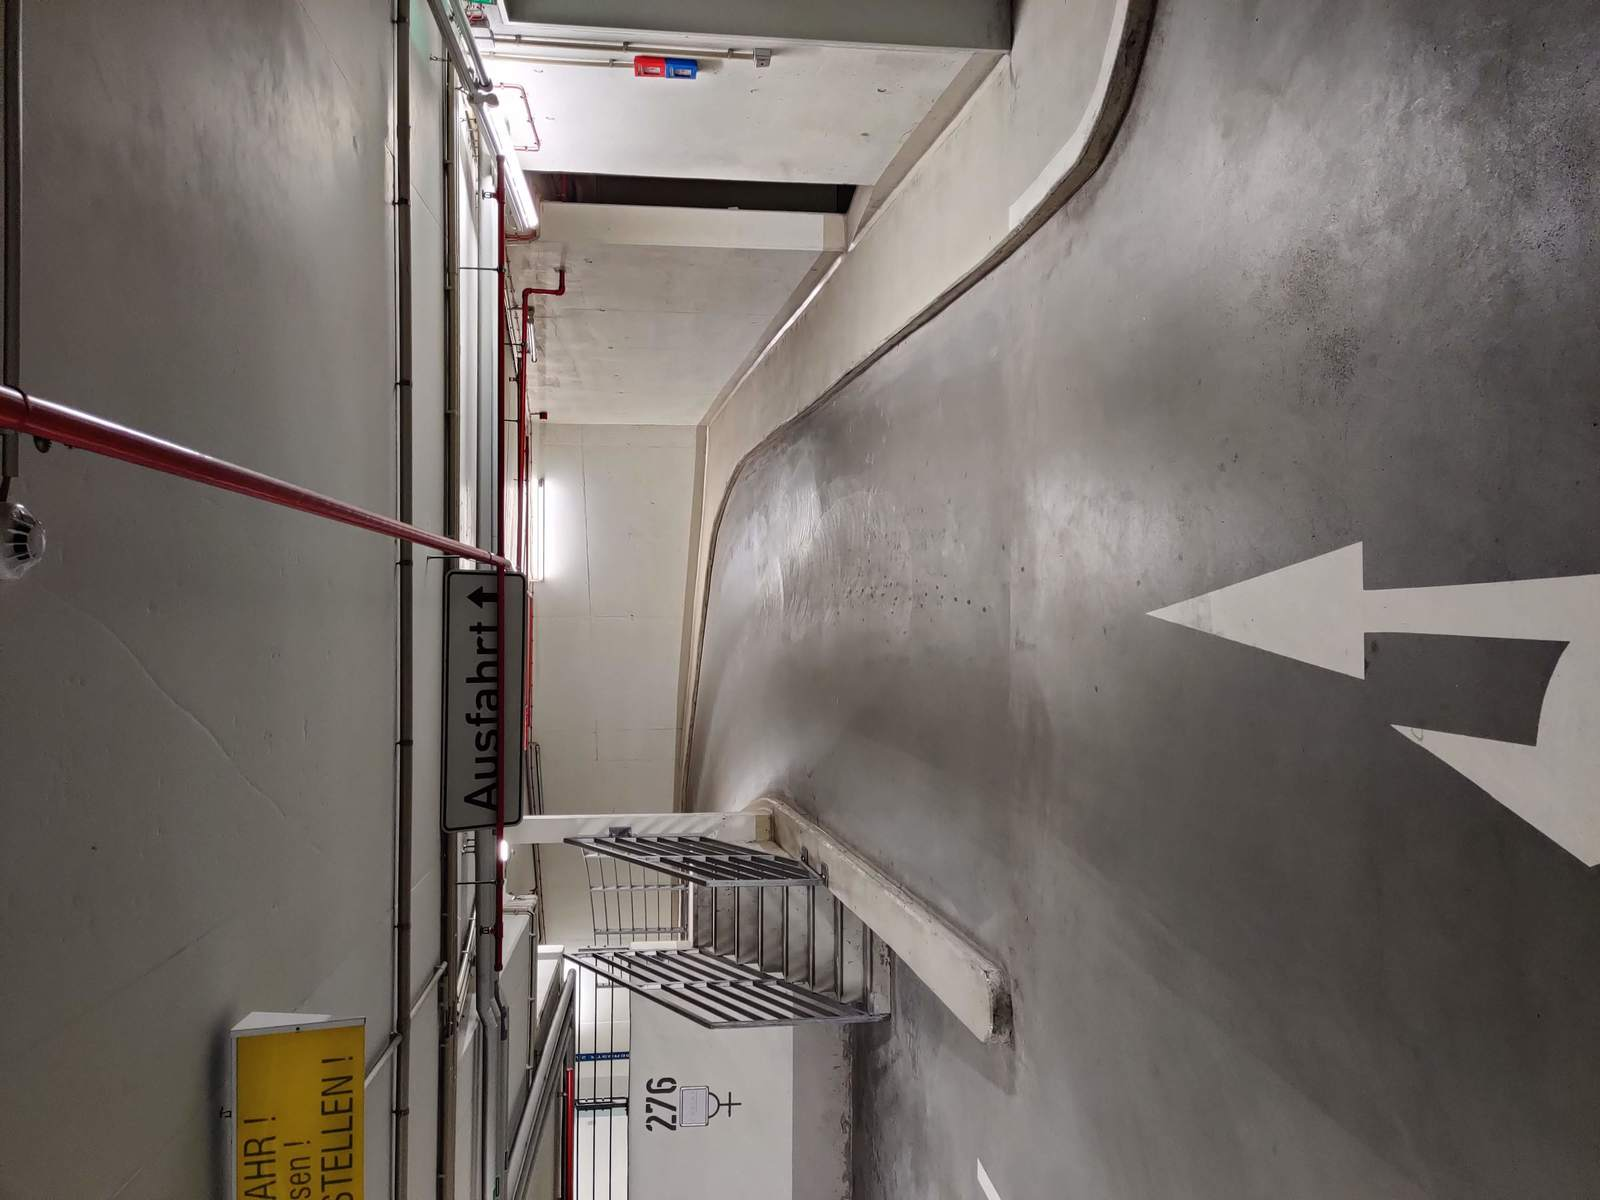
\includegraphics[angle=-90, width=1\linewidth]{RampB.jpg}
        \caption{}
    \end{subfigure}
    \hfill
    \begin{subfigure}{.24\linewidth}
        \centering
        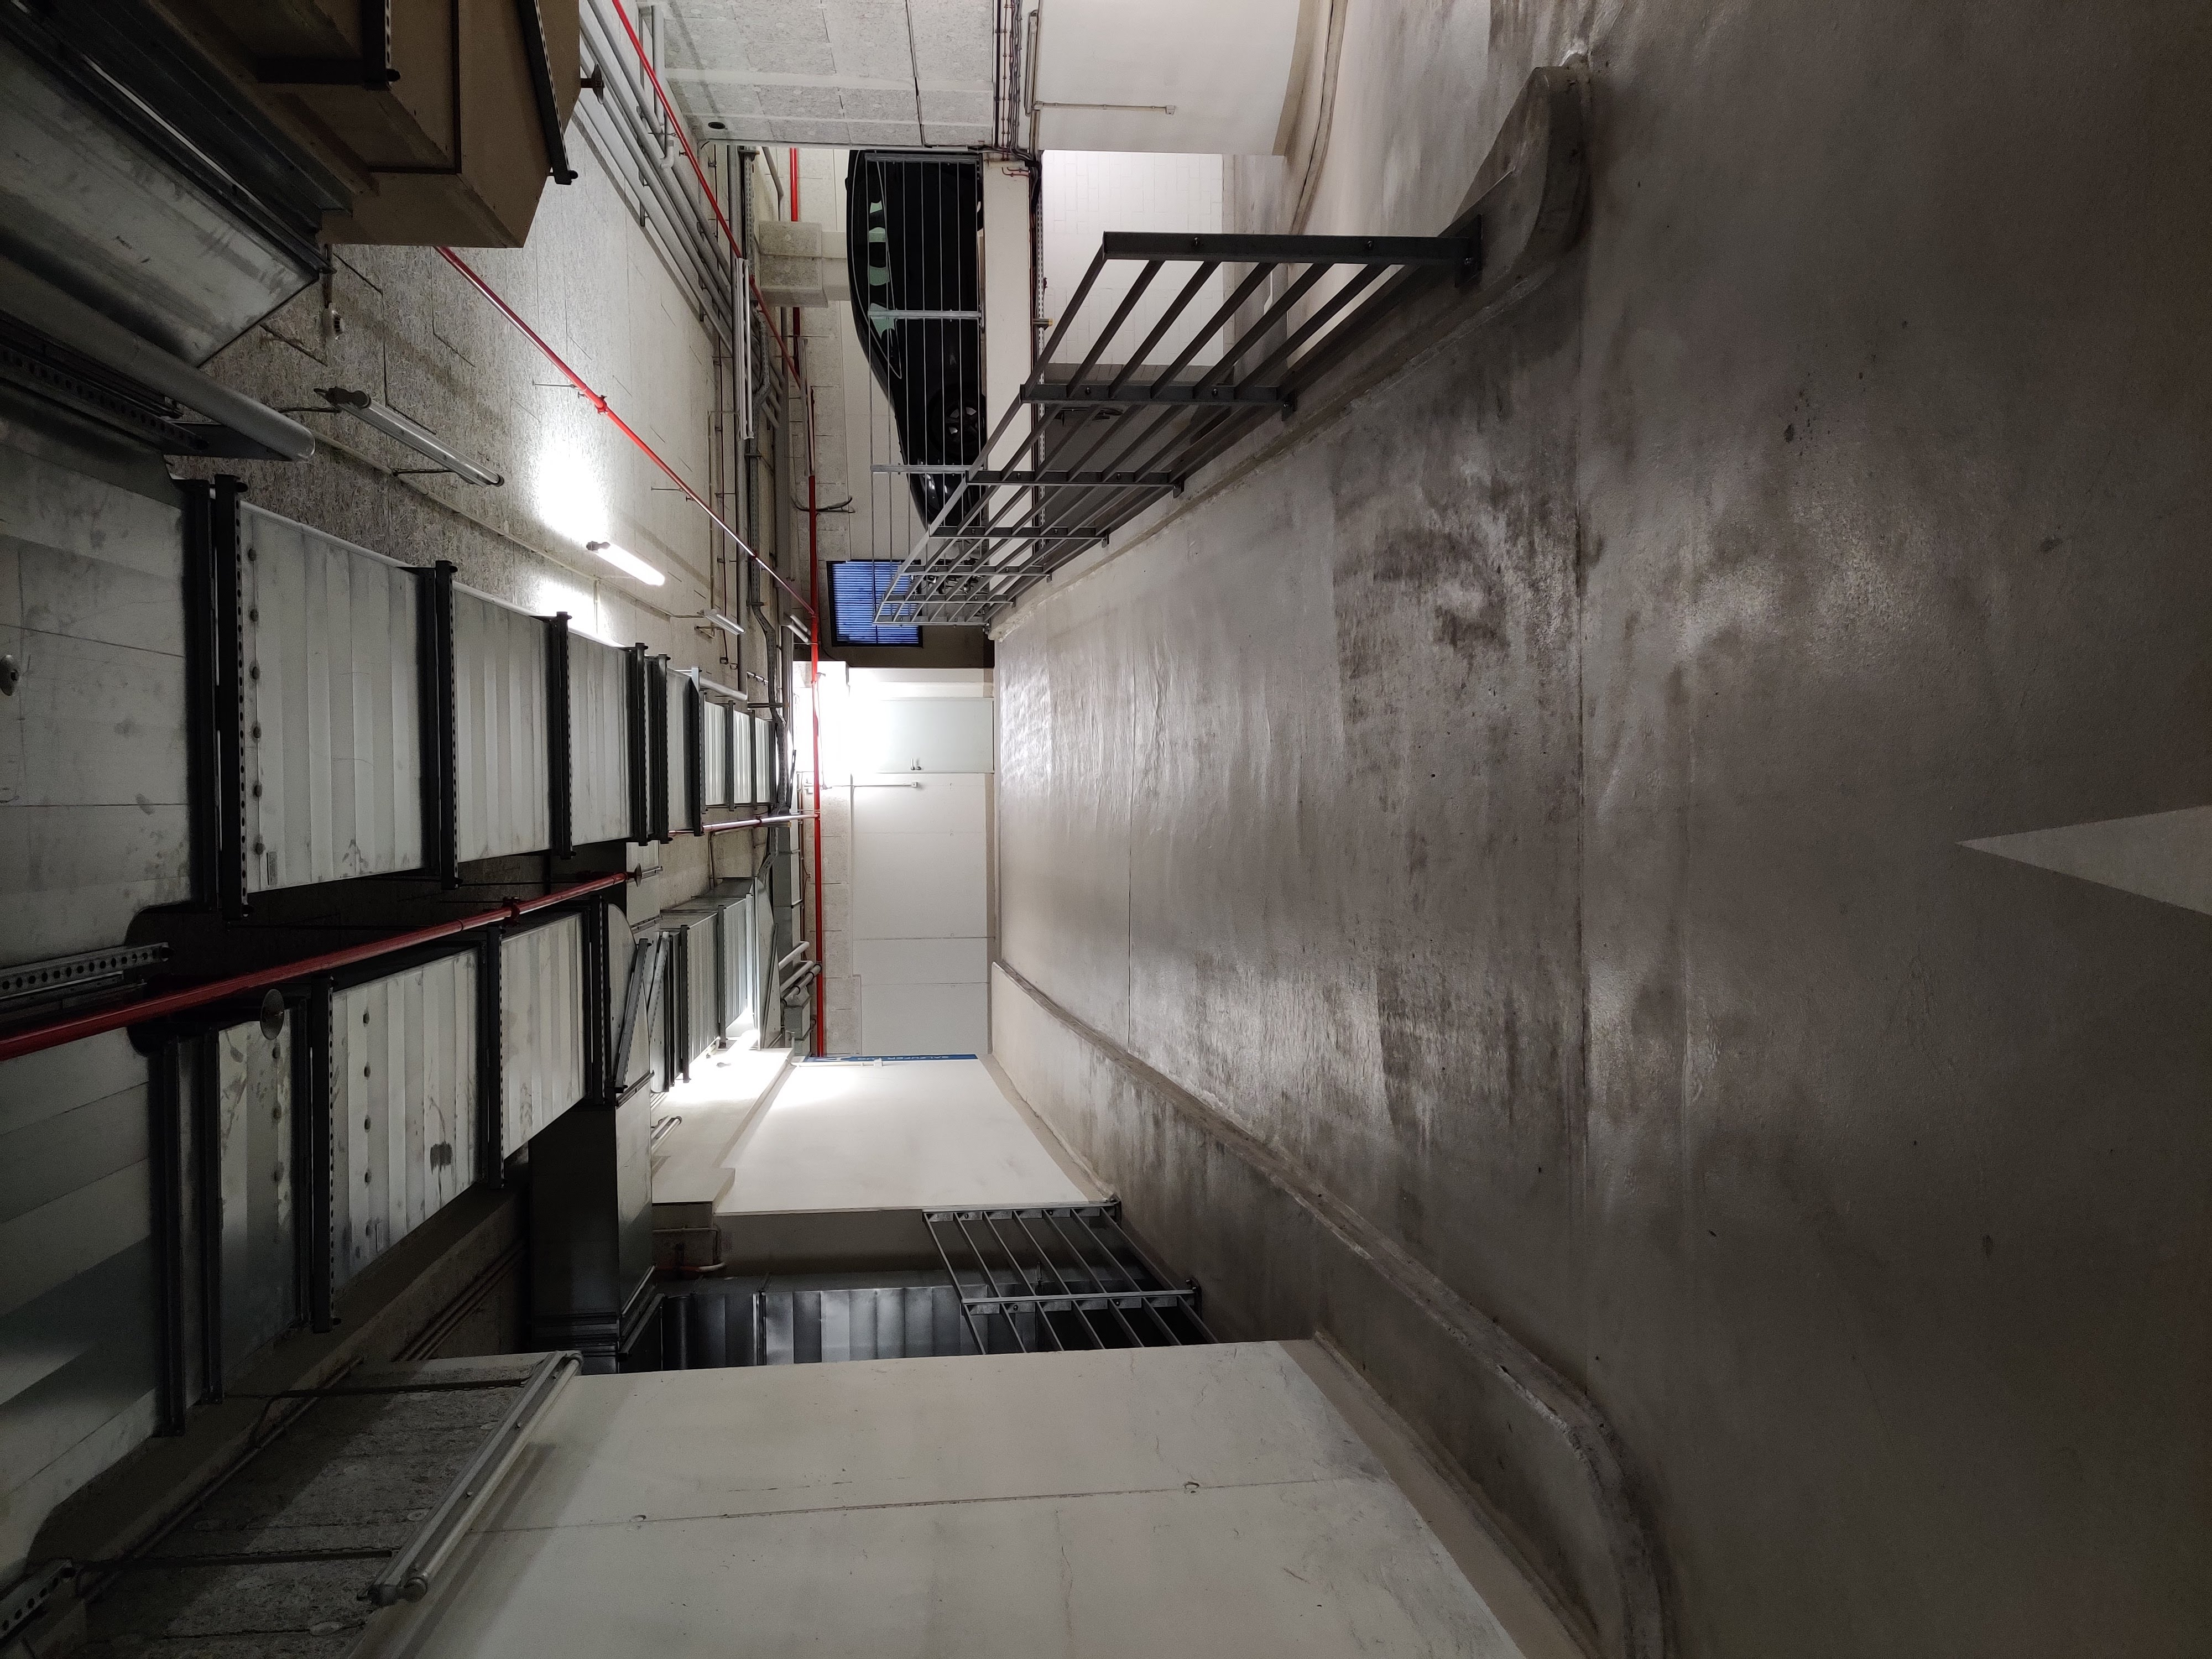
\includegraphics[width=1\linewidth]{RampC.jpg}
        \caption{}
    \end{subfigure}
    \hfill
    \begin{subfigure}{.24\linewidth}
        \centering
        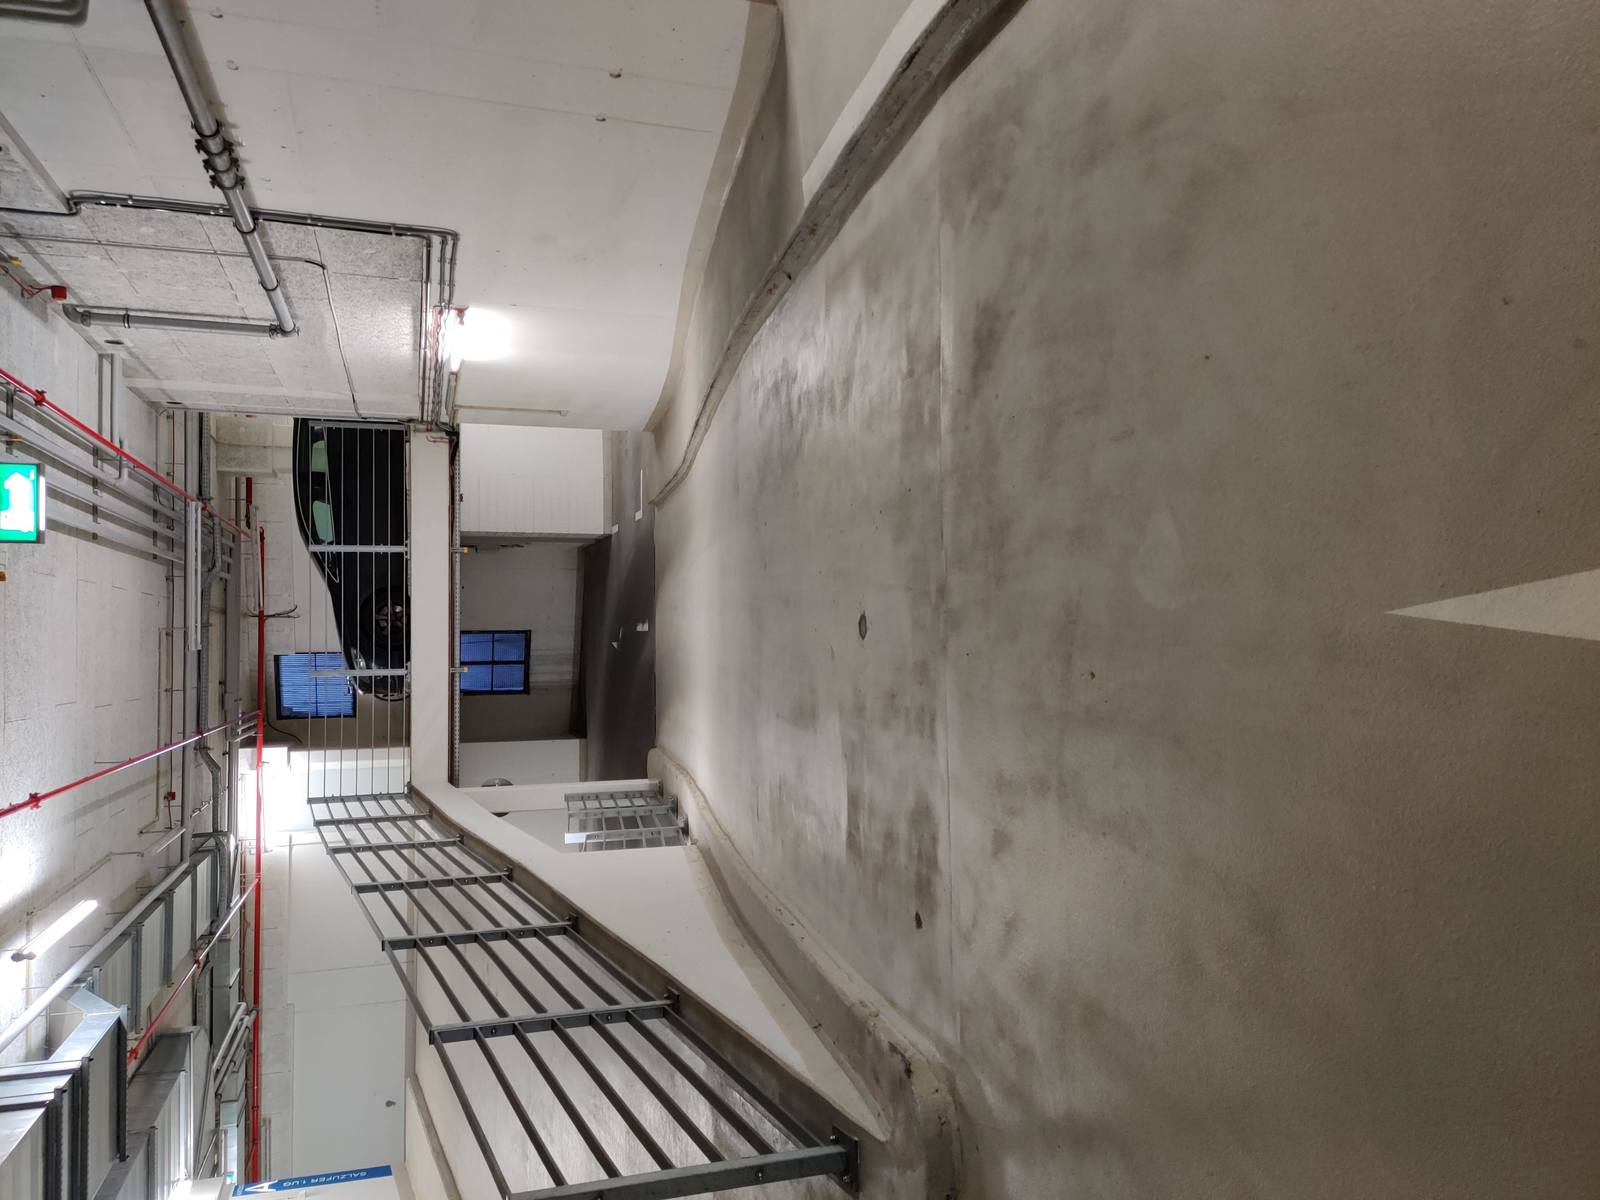
\includegraphics[angle=-90, width=1\linewidth]{RampD.jpg}
        \caption{}
    \end{subfigure}
    \caption[Ramps of the garage]{On the ramps A, B and C the car will be driven up. On the ramp D as well as also on the ramp A the car will be driven down.}
    \label{fig:all_ramps}
\end{figure}
\begin{table}[htb]
    \centering
    \caption[Measured ramp properties]{The measured ramp properties.}
    \label{tab:ramp_properties}
    \begin{tabular}[t]{cSSS}
        \toprule
        \textbf{Ramp} & {\textbf{Angle} [\si{\degree}]} & {\textbf{Width} [\si{\metre}]} & {\textbf{Length} [\si{\metre}]} \\
        \midrule
        A             & 7.2                             & 3.94                           & 11.97                           \\
        B             & 6.5                             & 3.96                           & 14.15                           \\
        C             & 7.4                             & 3.90                           & 11.85                           \\
        D             & -8.3                            & 3.85                           & 11.89                           \\
        \bottomrule
    \end{tabular}
\end{table}